% !TEX root = main.tex
In an online scenario, transmitter and receiver are assumed to have only causal information about energy arrivals i.e. they have no knowledge of future energy harvests. To model a general energy harvesting system, they are further assumed to not have any information about the distribution of future energy arrivals. We propose an algorithm to schedule the transmission of bits in this model. Motivated by \cite{VazeCompetitive}, we use competitive ratio analysis to compare the performance of online policy vs. the optimal offline policy. In this context, we say that our algorithm is $r$-competitive if for all possible energy arrivals at the transmitter $\ETx(t)$ and all possible `time' arrival $\TRx(t)$ at the receiver, the ratio of time taken by the online algorithm (say $T_{\mbox{\scriptsize{online}}}$) to the optimal offline one (say $T_{\mbox{\scriptsize{off}}}$) is bounded by $r$.
\begin{align}
&\displaystyle\max_{\ETx(t),\TRx(t)\hspace{0.5mm} \forall t}\dfrac{T_{\mbox{\scriptsize{online}}}}{T_{\mbox{\scriptsize{off}}}}\le r
\end{align}
 
\textit{Notation:} The starting time of transmission is denoted by $T_{\mbox{\scriptsize{start}}}$ and the present time is denoted by $t$. The number of bits and energy remaining to transmit at any transmitter energy epoch is represented by $B_{\mbox{\scriptsize{rem}}}$ and $E_{\mbox{\scriptsize{rem}}}$ receptively. We use the same notation $\{\bm{p},\bm{s},N\}$ to denote an onilne policy as described for offline policies.

The online algorithm that we propose is presented in Algorithm \ref{algo_online}. The Algorithm waits till time $T_{\mbox{\scriptsize{start}}}$ which marks the first energy arrival at transmitter or `time' addition at receiver such that using the energy $\ETx(T_{\mbox{\scriptsize{start}}})$ and time $\TRx(T_{\mbox{\scriptsize{start}}})$, $B_0$ or more bits can be transmitted.
\begin{equation}
T_{\mbox{\scriptsize{start}}}=\min\ t \ s.t.\  \TRx(t)g\Bigg{(} \dfrac{\ETx(t)}{\TRx(t)}\Bigg{)}\ge B_0.\label{online_T_start}
\end{equation}

To begin with, the transmitter equally divides $\ETx(T_{\mbox{\scriptsize{start}}})$ energy among all $B_0$ bits i.e. the first transmission power $p_1$ is set such that,
\begin{align}
&\frac{\ETx(T_{\mbox{\scriptsize{start}}})}{p_1}g(p_1)=B_0.
\label{eq_online_first_power}
\end{align}

By definition of $T_{\mbox{\scriptsize{start}}}$ in \eqref{online_T_start}, we know that transmission with power $p_1$ is going to finish in less than or equal to  $\TRx(T_{\mbox{\scriptsize{start}}})$ time.

If and when energy is harvested at the transmitter, the transmission power is changed. The total unused energy left at such an instant, $E_{\mbox{\scriptsize{rem}}}$, is equally divided among the bits left to transmit i.e. $B_{\mbox{\scriptsize{rem}}}$. Note that we do not change our transmission power when there is a `time' arrival at the receiver after $T_{\mbox{\scriptsize{start}}}$, because there is sufficient receiver time available to finish transmission. Also, the online algorithm changes its transmission power at every transmitter energy epoch after $T_{\mbox{\scriptsize{start}}}$ unlike the optimal offline policy. 

Fig. \ref{figure_online_example} shows output of Algorithm \ref{algo_online} for certain $\ETx(t)$ and $\TRx(t)$. Initially, suppose $B_0$ bits are not possible to be sent with $\ETx_0$ energy  within $\TRx_0$ time i.e. $\TRx(t_0)g\left( \dfrac{\ETx(t_0)}{\TRx(t_0)}\right)<B_0$. Further, $\TRx(r_1)g\left( \dfrac{\ETx(r_1)}{\TRx(r_1)}\right)<B_0$ and $\TRx(t_1)g\left( \dfrac{\ETx(t_1)}{\TRx(t_1)}\right)<B_0$. But, $\TRx(r_2)g\left( \dfrac{\ETx(r_2)}{\TRx(r_2)}\right)>B_0$. So, transmitter starts its transmission at $T_{\mbox{\scriptsize{start}}}=r_2$ with a power $p_1$ such that at rate $g(p_1)$, $B_0$ bits can be sent in $\ETx(r_2)/p_1$ time, as given in \eqref{eq_online_first_power}. At time $t=r_2$, transmitter expects transmission to finish by $r_2+\ETx(r_2)/p_1$ time. But, due to new energy arrival at time $t_2$, it can finish transmission earlier at a higher rate than $p_1$. At $t=t_2$, energy stored at transmitter is $E_{\mbox{\scriptsize{rem}}}=\ETx(r_2)+\ETx_2-(t_2-r_2)p_1$ and bits left to transmit is $B_{\mbox{\scriptsize{rem}}}=B_0-(t_2-r_2)g(p_1)$. Transmission power changes to $p_2$ at time $t_2$ such that $\frac{E_{\mbox{\scriptsize{rem}}}}{p_2}g(p_2)=B_{\mbox{\scriptsize{rem}}}$. Due to no new energy arrival till time $t_2+\frac{E_{\mbox{\scriptsize{rem}}}}{p_2}$, transmission completes at rate $p_2$, sending $B_0$ bits. 

\begin{figure}
\centering
  \centerline{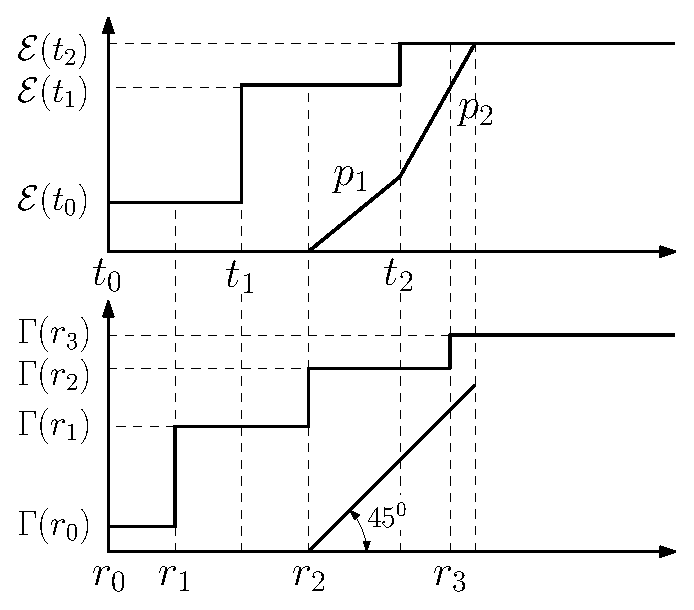
\includegraphics[width=8cm]{online.eps}}
\caption{Example showing execution of the online Algorithm \ref{algo_online}.}\label{figure_online_example}
\end{figure}


\begin{algorithm}
\caption {On-line Algorithm for energy harvesting transmitter and receiver.}
\footnotesize
\label{algo_online}
\begin{algorithmic}[1]
\State \textbf{Input}: Bits to transmit $B_0$; $\ETx_i$, $\TRx_i$ for $t_i,r_i<t$ where $t$ is the present time instant which increments parallely with this algorithm. 

\State $T_{\mbox{\scriptsize{start}}}=\min\ t$ s.t. $\TRx(t)g\Bigg{(} \dfrac{\ETx(t)}{\TRx(t)}\Bigg{)}\ge B_0$
\State $B_{\mbox{\scriptsize{rem}}}=B_0$, $E_{\mbox{\scriptsize{rem}}}=\ETx(T_{\mbox{\scriptsize{start}}})$, $m=T_{\mbox{\scriptsize{start}}}$

\Do
	\State Transmit at power $p$ such that $\dfrac{E_{\mbox{\scriptsize{rem}}}}{p} g(p)= B_{\mbox{\scriptsize{rem}}}$
	\If {$t=t_i$ for some $i$} 
		\State $B_{\mbox{\scriptsize{rem}}}=B_{\mbox{\scriptsize{rem}}}-(t_i-m)g(p)$
		\State $E_{\mbox{\scriptsize{rem}}}=E_{\mbox{\scriptsize{rem}}}+\ETx_i-(t_i-m)p$
		\State $m=t_i$
	\EndIf
\DoWhile {$t\le \left( m+\dfrac{E_{\mbox{\scriptsize{rem}}}}{p}\right)$}
\end{algorithmic}
\end{algorithm}

\begin{lemma}
The transmission power in the on-line algorithm is non-decreasing with time after $T_{start}$.
\label{online_power}
\end{lemma}
\begin{proof}
From the definition of the algorithm, the transmission power only changes when there is a new energy arrival at the transmitter, after $T_{\mbox{\scriptsize{start}}}$. 

So, if there is no new energy arrival after $T_{\mbox{\scriptsize{start}}}$, the transmit power is same ($=p_1$) i.e. non decreasing. 

Suppose there are energy arrivals after $T_{\mbox{\scriptsize{start}}}$ and for any energy arrival (say $E_{\mbox{\scriptsize{new}}}$) the power changes from $p_i$ to $p_{i+1}$. Let the energy remaining at start of transmission with power $p_i$ be $E_{\mbox{\scriptsize{rem}}}$ and bits remaining be $B_{\mbox{\scriptsize{rem}}}$. The transmission continues for time $l_i$ with power $p_i$. Now, we need to show that $p_i<p_{i+1}$. From the algorithm we get the following equations.  

\begin{align}
&\frac{g(p_i)}{p_i}=\frac{B_{\mbox{\scriptsize{rem}}}}{E_{\mbox{\scriptsize{rem}}}} \label{power_increasing_eq1}
\\
&\frac{g(p_{i+1})}{p_{i+1}}=\frac{B_{\mbox{\scriptsize{rem}}}-g(p_i) l_i}{E_{\mbox{\scriptsize{rem}}}+E_{\mbox{\scriptsize{new}}}-p_i l_i}\label{power_increasing_eq2}
\end{align}
Substituting $g(p_i)$ from (\ref{power_increasing_eq1}) into RHS of (\ref{power_increasing_eq2}), we can see that $\frac{g(p_i)}{p_i}>\frac{g(p_{i+1})}{p_{i+1}}$. Hence, by monotonicity of $g(p)/p$ from \eqref{property_decreasing}, we know that $p_i<p_{i+1}$.
\end{proof}

\begin{lemma}
The online policy starts atleast by the time the optimal offline policy ends (say $T_{\mbox{\scriptsize{off}}}$) i.e. $T_{\mbox{\scriptsize{start}}} <T_{\mbox{\scriptsize{off}}}$.
\label{onilne_time}
\end{lemma}

\begin{proof}
We will prove this by contradiction. Suppose $T_{\mbox{\scriptsize{start}}} \ge T_{\mbox{\scriptsize{off}}}$. From \eqref{online_T_start}, either $T_{\mbox{\scriptsize{start}}}=t_i$ for some $i$ and/or $T_{\mbox{\scriptsize{start}}}=r_j$ for some $j$.

If $T_{\mbox{\scriptsize{start}}}=t_i$, then as $T_{\mbox{\scriptsize{off}}}\le T_{\mbox{\scriptsize{start}}}$, the maximum energy that can be utilized by the offline policy is $\ETx(T_{\mbox{\scriptsize{start}}}^-)=\ETx(T_{\mbox{\scriptsize{start}}})-\ETx_i$. Note that the offline policy cannot use energy arrival $\ETx_i$, as using any finite amount of energy for 0 time cannot deliver any bits. 

If $T_{\mbox{\scriptsize{start}}}=r_j$, then the maximum time for which the receiver can be \textit{on} in the offline policy is $\TRx(T_{\mbox{\scriptsize{start}}}^-)=\TRx(T_{\mbox{\scriptsize{start}}})-\TRx_j$, as the offline policy has to finish at or before $T_{\mbox{\scriptsize{start}}}$. Note that, in the optimal offline policy, time for which the receiver is \textit{on} is given by $\displaystyle \sum_{i:p_i\neq 0}(s_{i+1}-s_i)$. 
%If $T_{\mbox{\scriptsize{start}}}\neq t_i$ or $T_{\mbox{\scriptsize{start}}}\neq r_j$ then, $\ETx(T_{\mbox{\scriptsize{start}}}^-)=\ETx(T_{\mbox{\scriptsize{start}}})$ or $\TRx(T_{\mbox{\scriptsize{start}}}^-)=\TRx(T_{\mbox{\scriptsize{start}}})$.

Now, the number of bits transmitted by the offline policy $\{\bm{p},\bm{s},N\}$ is given by,
\begin{align}
&\sum_{{\substack{i=1\\p_i\neq 0}}}^{i=N} g(p_i)(s_{i+1}-s_{i}),
\\
&\nonumber \stackrel{(a)}{\le}g\left(\frac{\displaystyle\sum_{i:p_i\neq 0}p_i(s_{i+1}-s_{i})}{\displaystyle\sum_{j:p_j\neq 0}(s_{j+1}-s_{j})}\right)\sum_{j:p_j\neq 0} (s_{j+1}-s_{j}),
\\
&\nonumber\stackrel{(b)}{\le} g\left( \frac{\displaystyle\sum_{i:p_i\neq 0} p_i(s_{i+1}-s_{i})}{\TRx(T_{\mbox{\scriptsize{start}}}^-)} \right)\TRx(T_{\mbox{\scriptsize{start}}}^-), 
\\
&\le g\left(\frac{\ETx(T_{\mbox{\scriptsize{start}}}^-)}{\TRx(T_{\mbox{\scriptsize{start}}}^-)}\right)\TRx(T_{\mbox{\scriptsize{start}}}^-)\stackrel{(c)}{<}B_0.\label{online_eq_2}
\end{align}
%%%&\nonumber\stackrel{(a)}{\le} g\left(\sum_{\substack{i\\p_i\neq 0}}p_i\left(\frac{(s_{i+1}-s_{i})}{\displaystyle\sum_{j:p_j\neq 0}(s_{j+1}-s_{j})}\right)\right) \sum_{\substack{j\\p_j\neq 0}} (s_{j+1}-s_{j}),

where $(a)$ follows from application of Jensen's inequality due to concavity of $g(p)$; $(b)$ follows form the fact that $\displaystyle\sum_{j:p_j\neq 0}(s_{j+1}-s_{j})\le\TRx(s_{N+1})\le \TRx(T_{\mbox{\scriptsize{start}}}^-)$ and $g(p)/p$ is monotonically decreasing; $(c)$ follows form \eqref{online_T_start}. \eqref{online_eq_2} implies that the number of bits transmitted by the offline policy is less than $B_0$. Hence, it amounts to a contradiction and therefore, $T_{\mbox{\scriptsize{start}}}<T_{\mbox{\scriptsize{off}}}$.
\end{proof}
\begin{lemma}
In the optimal online policy $\{\bm{p},\bm{s},N\}$, if $p_i$ is the transmission power at time $t$ then $\dfrac{p_i}{g(p_i)} \ge \dfrac{\ETx(t)}{B_0}\;\;\forall\;\; T_{\mbox{\scriptsize{start}}}\le t\le T_{\mbox{\scriptsize{online}}}$
\end{lemma}
\begin{proof}
First we shall prove that this result holds for $t\in S$ where $S$ is the ordered set $\{T_{\mbox{\scriptsize{start}}},t_k,t_{k+1},...,t_l\}$ where $t_i's$ are the transmitter energy arrival epochs. $t_k$ is the first energy arrival epoch after $T_{\mbox{\scriptsize{start}}}$ and $t_l$ is the last one before $T_{\mbox{\scriptsize{online}}}$. 
We will prove our result this by induction. In the base case, when $t = T_{\mbox{\scriptsize{start}}}$, by our allocation algorithm,
\begin{equation}
\dfrac{p_i}{g(p_i)} = \dfrac{p_1}{g(p_1)} = \dfrac{\ETx(T_{\mbox{\scriptsize{start}}})}{B_0}.
\end{equation}
So our result holds true. Now for the induction step, assume that the result is true for all $t_i<t_m$ in $S$. Note that at any time, $\dfrac{p_i}{g(p_i)} = \dfrac{\ETx(T_{\mbox{\scriptsize{start}}})}{B_{\mbox{\scriptsize{start}}}}$. Let $E_{\mbox{\scriptsize{rem}}}$ and $B_{\mbox{\scriptsize{rem}}}$ represent the remaining transmitter energy and bits to transfer at $t_{m-1}$. Let  $E_{\mbox{\scriptsize{rem}}}'$ and $B_{\mbox{\scriptsize{rem}}}'$ be the remaining energy and bits at time $t_m$. 
\begin{align}
&\dfrac{E_{\mbox{\scriptsize{rem}}}'}{B_{\mbox{\scriptsize{rem}}}'} = \dfrac{E_{\mbox{\scriptsize{rem}}} + \ETx_m - p_{i-1}l_{i-1}}{B_{\mbox{\scriptsize{rem}}} - g(p_{i-1}l_{i-1},
&\dfrac{E_{\mbox{\scriptsize{rem}}}'}{B_{\mbox{\scriptsize{rem}}}'} = \dfrac{E_{\mbox{\scriptsize{rem}}} + \ETx_m - \frac{E_{\mbox{\scriptsize{rem}}}}{B_{\mbox{\scriptsize{rem}}}}}{B_{\mbox{\scriptsize{rem}}} - \frac{E_{\mbox{\scriptsize{rem}}}}{B_{\mbox{\scriptsize{rem}}}}},
\end{align}
\end{proof}


\begin{theorem}
The competitive ratio of the online policy presented in Algorithm \ref{algo_online} is strictly less than 2.
\end{theorem}
\begin{proof}
This is equivalent to saying that the time taken by the online policy can at max be approaching twice the time taken by optimal offline policy, over all possible energy arrival sequences. Let the time taken by the optimal offline policy be $T_{\mbox{\scriptsize{off}}}$ and the online policy, say $\{\bm{{p}},\bm{{s}},{N}\}$, be $T_{\mbox{\scriptsize{online}}}$. Note that $s_{N+1}=T_{\mbox{\scriptsize{online}}}$. 

The idea behind the proof is to show that the online policy can conitnue for at max $T_{\mbox{\scriptsize{off}}}$ time  after the offline policy ends.
%
%If $T_{\mbox{\scriptsize{start}}}=r_j$, then then the maximum time for which the receiver can be \textit{on} is $\TRx(T_{\mbox{\scriptsize{start}}}^-)=\TRx(T_{\mbox{\scriptsize{start}}})-\TRx_j$, as the offline policy has to finish at or before $T_{\mbox{\scriptsize{start}}}$.
%Now, from \eqref{online_eq_4}, the maximum number of bits being transmitted can be bounded by  
%\begin{align}
%&=g\left(\frac{\displaystyle\sum_{i=1}^{i=N}p_i(s_{i+1}-s_{i})}{(s_{N+1}-s_{1})}\right)(s_{N+1}-s_{1}),
%\\
%&=g\left(\frac{\ETx(T_{\mbox{\scriptsize{start}}}}{\TRx(T_{\mbox{\scriptsize{start}}}^-)}\right)\TRx(T_{\mbox{\scriptsize{start}}}^-),
%\\
%&=g\left(\frac{\ETx(T_{\mbox{\scriptsize{start}}}}{\TRx(T_{\mbox{\scriptsize{start}}})-\TRx_j}\right)(\TRx(T_{\mbox{\scriptsize{start}}})-\TRx_j)<B_0
%\label{online_eq_5}
%\end{align}
%where \eqref{online_eq_5} again follows form \eqref{online_T_start}.

Consider the transmission power of the online policy just before $T_{\mbox{\scriptsize{off}}}$. Let this be ${p}_l$. As $T_{\mbox{\scriptsize{start}}}<T_{\mbox{\scriptsize{off}}}$ from Lemma \ref{onilne_time}, such a power will always exist and $s_l<T_{\mbox{\scriptsize{off}}}$. Let $E_{\mbox{\scriptsize{rem}}}$ and $B_{\mbox{\scriptsize{rem}}}$ denote the residual energy and bits at time ${s}_{l}$. Note that, either ${s}_{l}=T_{\mbox{\scriptsize{start}}}$ or ${s}_{l}=t_k$ for some $k$. Also, 
\begin{align}
&\ETx({s}_{l})=\ETx(T_{\mbox{\scriptsize{off}}}),
\label{eq_online_time_0}
\end{align}
because if $T=t_k$, $t_k$ would be the last energy arrival epoch before $T_{\mbox{\scriptsize{off}}}$ or $T=T_{\mbox{\scriptsize{start}}}$, then $T_{\mbox{\scriptsize{start}}}$ would be greater than the last energy arrival epoch before $T_{\mbox{\scriptsize{off}}}$. 

Since the number of bits sent by online policy after ${s}_l$ is equal to $B_{\mbox{\scriptsize{rem}}}$, by Lemma \ref{online_power},
\begin{align}
&\sum_{i=l}^{i={N}}g(p_i)({s}_{i+1}-{s}_i)=B_{\mbox{\scriptsize{rem}}},
\\
&({s}_{{N}+1}-{s}_l)\le\frac{B_{\mbox{\scriptsize{rem}}}}{g(p_l)}=\frac{E_{\mbox{\scriptsize{rem}}}}{p_l}\le \frac{\ETx({s}_l)}{p_l}.
\label{eq_online_time_1}  
\end{align}
Applying Lemma \ref{lemma_online_inequality} on $p_l$ and using \eqref{eq_online_time_0},
\begin{align}
&\frac{\ETx(T_{\mbox{\scriptsize{off}}})}{p_l}g(p_l)=\frac{\ETx({s}_l)}{p_l}g(p_l)\le B_0\stackrel{(a)}{\le}T_{\mbox{\scriptsize{off}}}\; g\left(\frac{\ETx(T_{\mbox{\scriptsize{off}}})}{T_{\mbox{\scriptsize{off}}}}\right)
\label{eq_online_time_2}
\end{align}
where $(a)$ holds because the maximum bits sent by the offline policy can be bounded by $T_{\mbox{\scriptsize{off}}}\; g\left(\frac{\ETx(T_{\mbox{\scriptsize{off}}})}{T_{\mbox{\scriptsize{off}}}}\right)$. By monotonicity property of $g(p)/p$ in \eqref{property_decreasing}, we can conclude from \eqref{eq_online_time_2} that, $\frac{\ETx({s}_l)}{p_l}=\frac{\ETx(T_{\mbox{\scriptsize{off}}})}{p_l}\le T_{\mbox{\scriptsize{off}}}$. Combining this with \eqref{eq_online_time_1}, we get,
\begin{align}
&({s}_{{N}+1}-{s}_l)\le T_{\mbox{\scriptsize{off}}}.
\label{eq_online_time_3}
\end{align} 

Finally, we can calculate the competitive ratio for Algorithm \ref{algo_online} as,
\begin{align*}
&r=\displaystyle\max_{\ETx(t),\TRx(t)\hspace{0.5mm} \forall t}\dfrac{T_{\mbox{\scriptsize{online}}}}{T_{\mbox{\scriptsize{off}}}} = \dfrac{({s}_{{N}+1}-{s}_l)+{s}_l}{T_{\mbox{\scriptsize{off}}}} \stackrel{(a)}{<} 2,
\end{align*}
where $(a)$ follows from \eqref{eq_online_time_3}, and ${s}_l<T_{\mbox{\scriptsize{off}}}$.        
\end{proof}
